\chapter{Sistema Proposto}
\label{chap:sistema_proposto}

A solução proposta visa anteder inicialmente os membros NAPI Abelhas, podendo em etapa futura atender outros grupos de pesquisadores do Brasil e do Mundo, de diferentes instituições. Será necessário registrar dados de pesquisadores, produtores e técnicos responsáveis por cada amostra, mas como usuário do sistema, na sua versão proposta neste documento, irá existir apenas um perfil de usuário administrador, referente a função do técnico responsável.

A solução foi projetada para atender uma das principais demandas dos pesquisadores do NAPI Abelhas, focando na integridade dos dados, na rastreabilidade e na eficiência do fluxo de trabalho. A seguir, são detalhados os requisitos e a arquitetura do sistema.

\section{Requisitos}
\label{sec:requisitos}

\subsection{Requisitos Funcionais}

As funcionalidades do sistema foram estruturadas em módulos lógicos para cobrir o fluxo operacional do laboratório e as necessidades administrativas do NAPI Abelhas.

\begin{itemize}
    \item \textbf{Módulo de Gestão Administrativa:}
    \begin{itemize}
        \item \textbf{Controle de Acesso e Identidade:}  O sistema garante que apenas usuários autorizados (Responsáveis Técnicos) acessem as funcionalidades de escrita, mantendo um registro auditável de quem realizou cada operação (vínculo com a entidade \textit{Responsável}).
        Integração com o serviço externo \textit{Clerk}\footnote{Uma plataforma autenticação e gerenciamento de usuário: https://clerk.com/} para autenticação segura.
        
        \item \textbf{Gestão de Produtores e Pontos de Coleta:} Funcionalidade de cadastro completo de apicultores e meliponicultores. Inclui o registro georreferenciado (latitude, longitude e raio) dos apiários (\textit{ponto de coleta} das amostras), permitindo a correlação futura entre informações obtidas das amostras e suas respectiva região de origem, viabilizando a execução de pesquisas relacionadas a certificação de origem geográfica do mel produzido e identificação de condições atípicas/sazonais, que impactam na produção do mel em micro e macro regiões.
    \end{itemize}
    
    \item \textbf{Módulo para Gestão das Amostras e Análises:}
    \begin{itemize}
        \item \textbf{Recepção e Rastreabilidade (Check-in):} Processo de digitalização da entrada da amostra física produzidas pelo NAPI. O sistema gera um identificador único (UUID) para a entidade \textit{Amostra}, vinculando-a obrigatoriamente a um produtor, a um ponto de coleta, a uma espécie de abelha, a um tipo de amostra e a imagens relacionadas, e ao local onde essas amostras estão armazenadas, estabelecendo a base para a rastreabilidade total.
        \item \textbf{Gerenciamento de Análises:} Interface para a criação e acompanhamento de das análises físico-químicas realizadas. O sistema permite atribuir múltiplos tipos de exames vinculados a cada amostra, sendo que para cada um diferente tipo de arquivo com seus resultados serão armazenados no sistema. Será utilizado um padrão de \textit{Pre-signed URLs} para realizar uploads diretos e seguros para o \textit{Object Storage} (MinIO), garantindo que documentos pesados não impactem a performance da API.
    \end{itemize}
    \item \textbf{Módulo de Consultas:}
    \begin{itemize}
        %\item \textbf{Gestão Documental (Upload Seguro):} Mecanismo para envio de arquivos de laudos e evidências visuais.
        \item \textbf{Consultas com filtros:} deve ser possível consultar os dados cadastrados, com filtros relacionados ao produto, tipo de amostra, período, status, entre outros.
        
         %Ferramenta de busca avançada que permite localizar amostras por produtor, período ou status. Facilita a recuperação de laudos antigos armazenados na tabela \textit{File}, servindo como repositório centralizado de informações do NAPI.
    \end{itemize}
\end{itemize}

\subsection{Requisitos Não-Funcionais}

Os requisitos não-funcionais definem os atributos de qualidade e as restrições técnicas da solução proposta:

\begin{itemize}
    \item \textbf{Segurança:} para garantir um acesso seguro aos dados, a aplicação proposta não irá armazenar senhas localmente, delegando a autenticação ao uso de tokens JWT. O acesso aos arquivos de laudos será protegido por URLs assinadas temporárias, com tempo de expiração reduzido para visualização.

    \item \textbf{Desempenho (Performance):} com o crescimento progressivo do número de usuários — envolvendo inicialmente pesquisadores de todo o estado — o sistema deve apresentar desempenho capaz de suportar um aumento de acessos a médio prazo. Para isso, o sistema proposto utilizará uma estratégia \textit{Cache-First} (Redis) para dados de leitura frequente e baixa volatilidade (como listas de cidades, espécies de abelhas e tipos de análise), reduzindo a latência da interface.

    \item \textbf{Escalabilidade e Portabilidade:} existe a necessidade de que a aplicação possa ser implantada, atualizada e ampliada de maneira eficiente, acompanhando o aumento da demanda e possíveis mudanças de infraestrutura. Para tal, a arquitetura será integralmente baseada em contêineres (Docker), permitindo que a API, o banco de dados e os serviços de suporte sejam implantados e escalados de forma independente em qualquer ambiente compatível.

\end{itemize}


\section{Tecnologias Utilizadas}
\label{sec:tecnologias}

A seleção tecnológica priorizou ferramentas de código aberto, robustas e amplamente adotadas pelo mercado, visando atender aos requisitos de desempenho e escalabilidade do projeto.

\begin{itemize}
    \item \textbf{Linguagem e Runtime:}
        \begin{itemize}
            \item \textbf{Node.js:} Ambiente de execução JavaScript assíncrono e orientado a eventos, construído sobre o motor V8 do Google Chrome, ideal para aplicações escaláveis de rede \cite{casciaro2020}.
            \item \textbf{TypeScript:} Superconjunto do JavaScript que adiciona tipagem estática opcional à linguagem, proporcionando maior segurança no desenvolvimento e facilidade na manutenção do código \cite{cherny2019}.
        \end{itemize}

    \item \textbf{Frontend:}
        \begin{itemize}
            \item \textbf{React:} Biblioteca JavaScript declarativa, eficiente e flexível para a construção de interfaces de usuário baseadas em componentes \cite{banks2020}.
            \item \textbf{Vite:} Ferramenta de construção (\textit{build tool}) que utiliza o suporte nativo a módulos ES (ESM) para oferecer um ambiente de desenvolvimento com recarregamento rápido e otimizado \cite{vite2024}.
        \end{itemize}

    \item \textbf{Persistência:}
        \begin{itemize}
            \item \textbf{PostgreSQL:} Sistema gerenciador de banco de dados objeto-relacional (ORDBMS) de código aberto, reconhecido por sua robustez, conformidade com padrões ACID e extensibilidade \cite{postgres2024}.
            \item \textbf{Prisma ORM:} Mapeador objeto-relacional moderno que oferece segurança de tipos (\textit{type-safety}) e gerencia migrações de esquema de forma declarativa \cite{prisma2024}.
        \end{itemize}

    \item \textbf{Armazenamento e Cache:}
        \begin{itemize}
            \item \textbf{MinIO:} Servidor de armazenamento de objetos de alto desempenho, compatível com a API Amazon S3, utilizado para persistência segura de arquivos não estruturados \cite{minio2024}.
            \item \textbf{Redis:} Armazenamento de estrutura de dados em memória, utilizado como banco de dados, cache e \textit{message broker} para otimização de latência \cite{redis2024}.
        \end{itemize}

    \item \textbf{Segurança e Infraestrutura:}
        \begin{itemize}
            \item \textbf{Clerk:} Solução completa de gerenciamento de identidade e acesso (IAM), fornecendo autenticação segura e gestão de sessões de usuário \cite{clerk2024}.
            \item \textbf{Docker:} Plataforma de software para desenvolvimento, envio e execução de aplicações dentro de contêineres, garantindo isolamento e portabilidade entre ambientes \cite{poulton2023}.
        \end{itemize}
\end{itemize}

\section{Arquitetura Proposta}
\label{sec:arquitetura}
A arquitetura da solução segue o modelo de serviços desacoplados, visando escalabilidade e facilidade de manutenção. A Figura \ref{fig:arquitetura} ilustra a visão geral dos componentes e suas interações.

O \textit{Frontend} (React) atua como cliente consumidor, comunicando-se com a API Backend para operações transacionais e interagindo diretamente com o \textit{Object Storage} (MinIO) para a transferência de arquivos binários, otimizando o tráfego de rede.

\begin{figure}[H]
    \centering
    \caption{Visão Geral da Arquitetura do Sistema}
    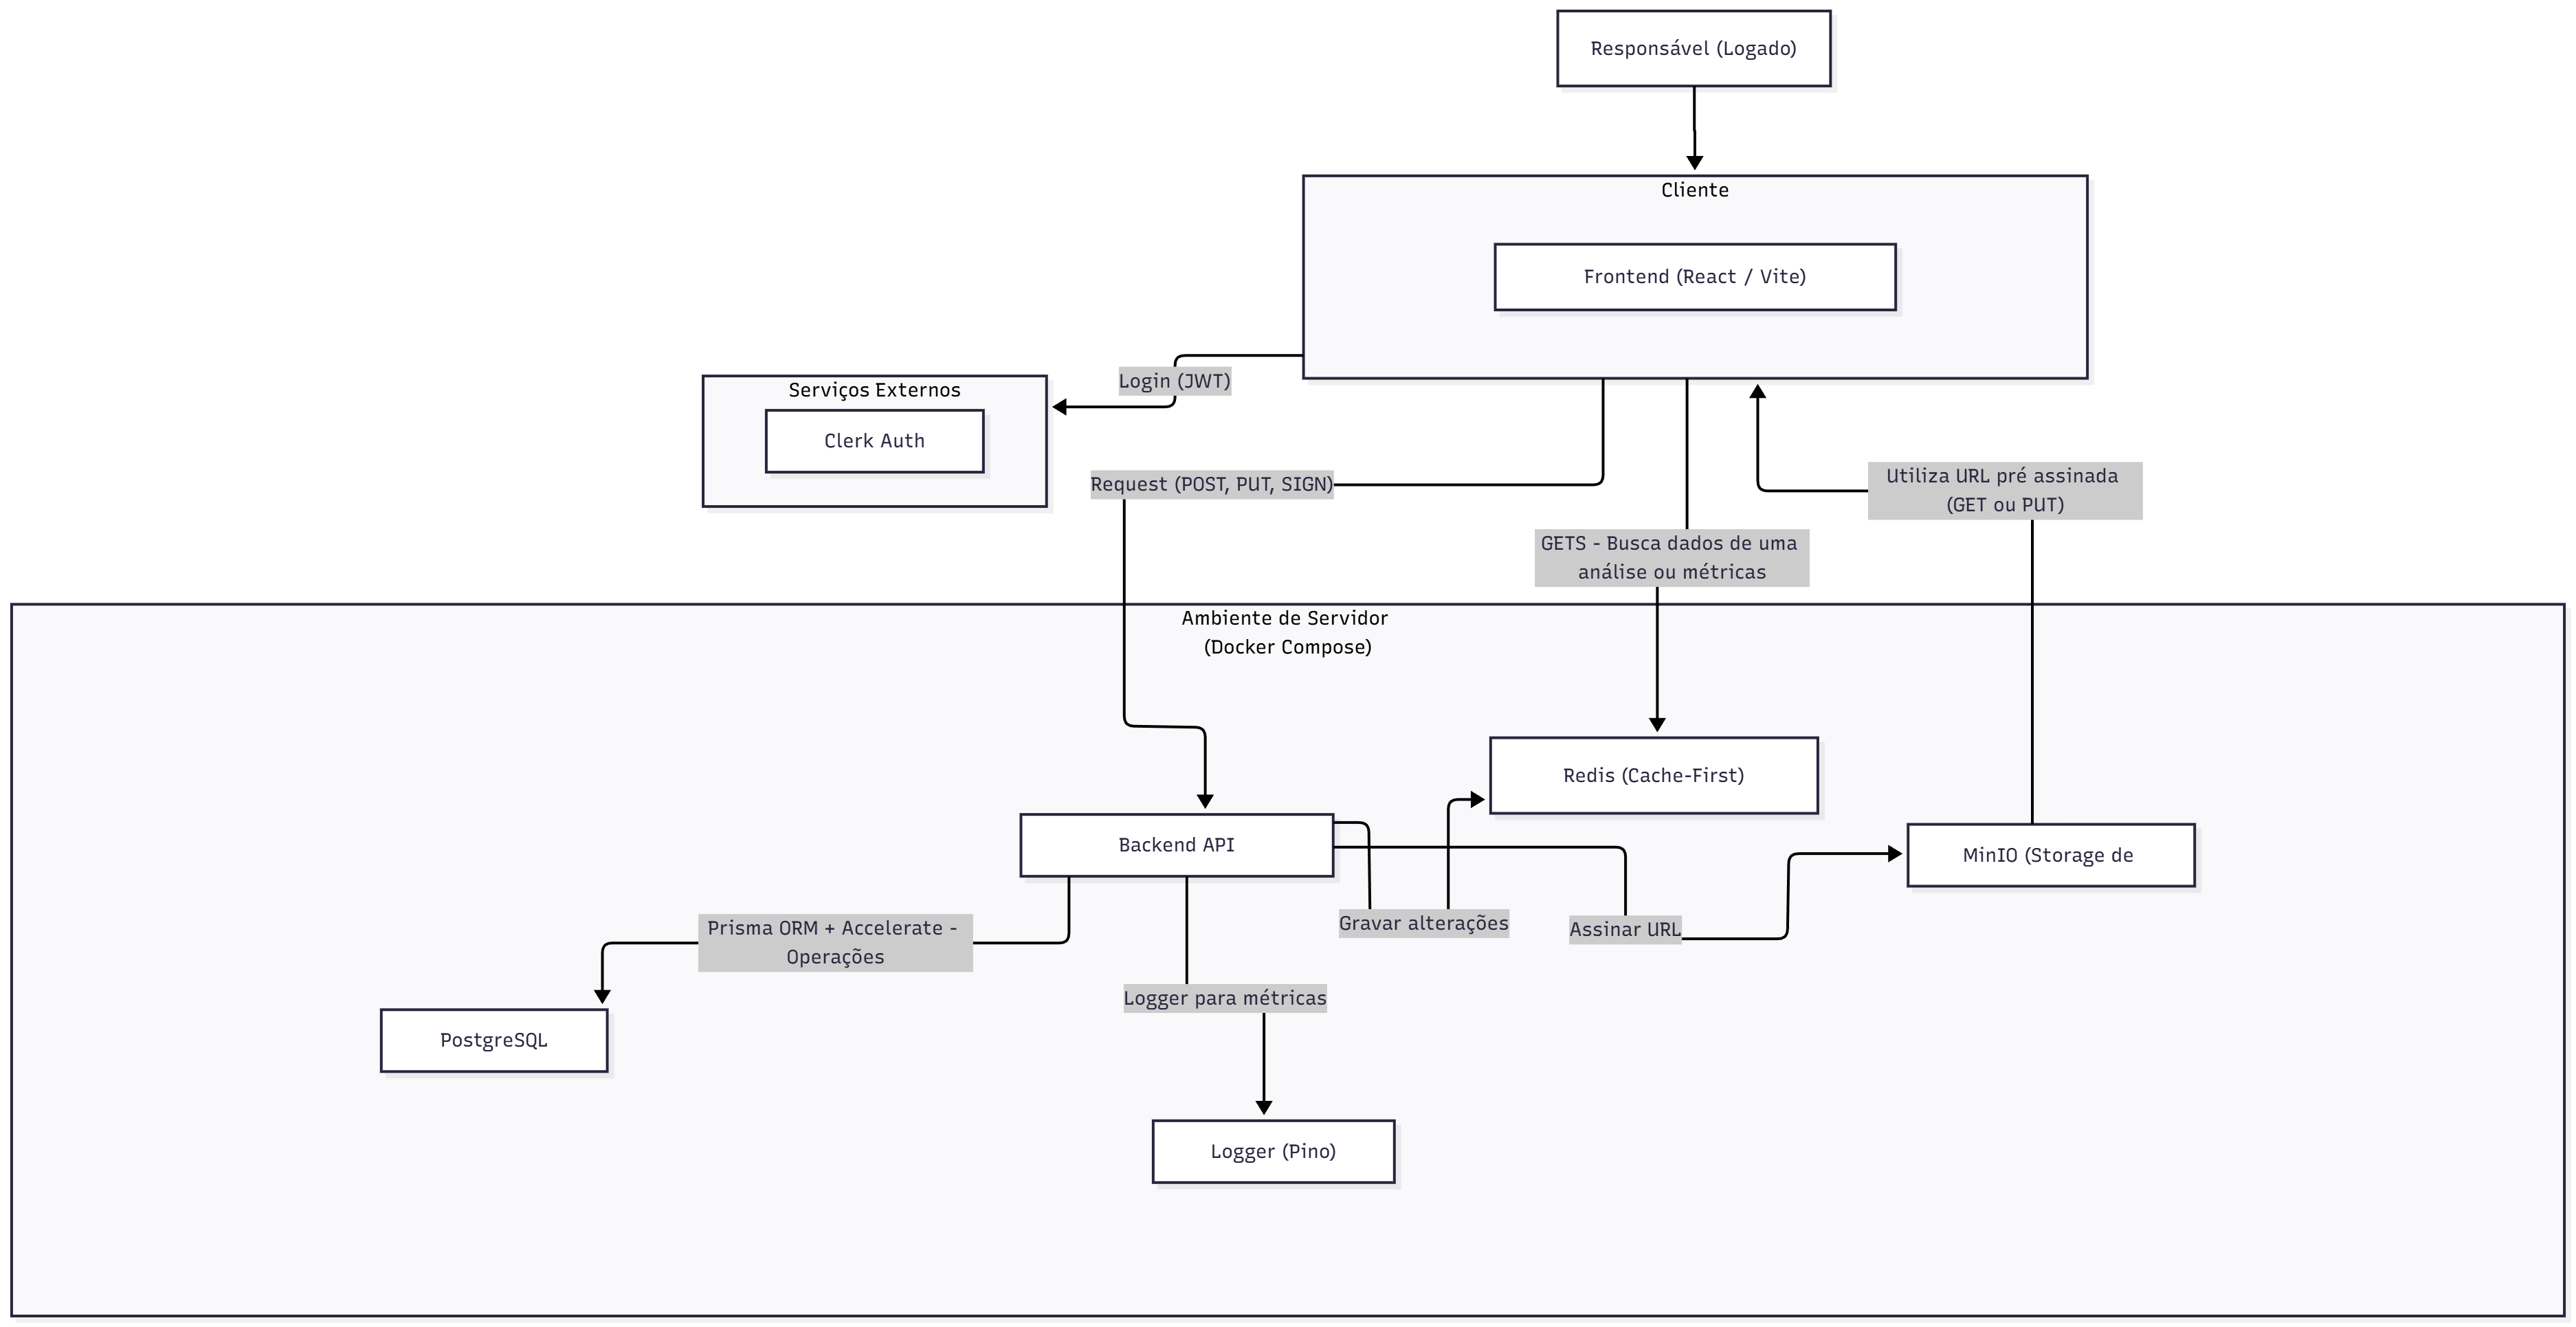
\includegraphics[width=1.0\textwidth]{Imagens/diagramaArquitetura.png}
    \fonte{Autoria própria (2025).}
    \label{fig:arquitetura}
\end{figure}

\section{Persistência de Dados}
\label{sec:persistencia}

A persistência adota uma abordagem híbrida: dados estruturados relacionais para garantir a integridade do negócio e armazenamento de objetos para arquivos binários. A Figura \ref{fig:der} apresenta o Modelo Lógico do Banco de Dados.

Entidades principais como \textit{Amostra}, \textit{Produtor} e \textit{Análise} são mantidas no PostgreSQL para garantir integridade referencial estrita, enquanto as tabelas \textit{File} e \textit{FileGroup} gerenciam apenas os metadados e ponteiros para os arquivos físicos salvos no \textit{Storage}.

\begin{figure}
    \centering
    \caption{Diagrama Entidade-Relacionamento (DER) Lógico}
    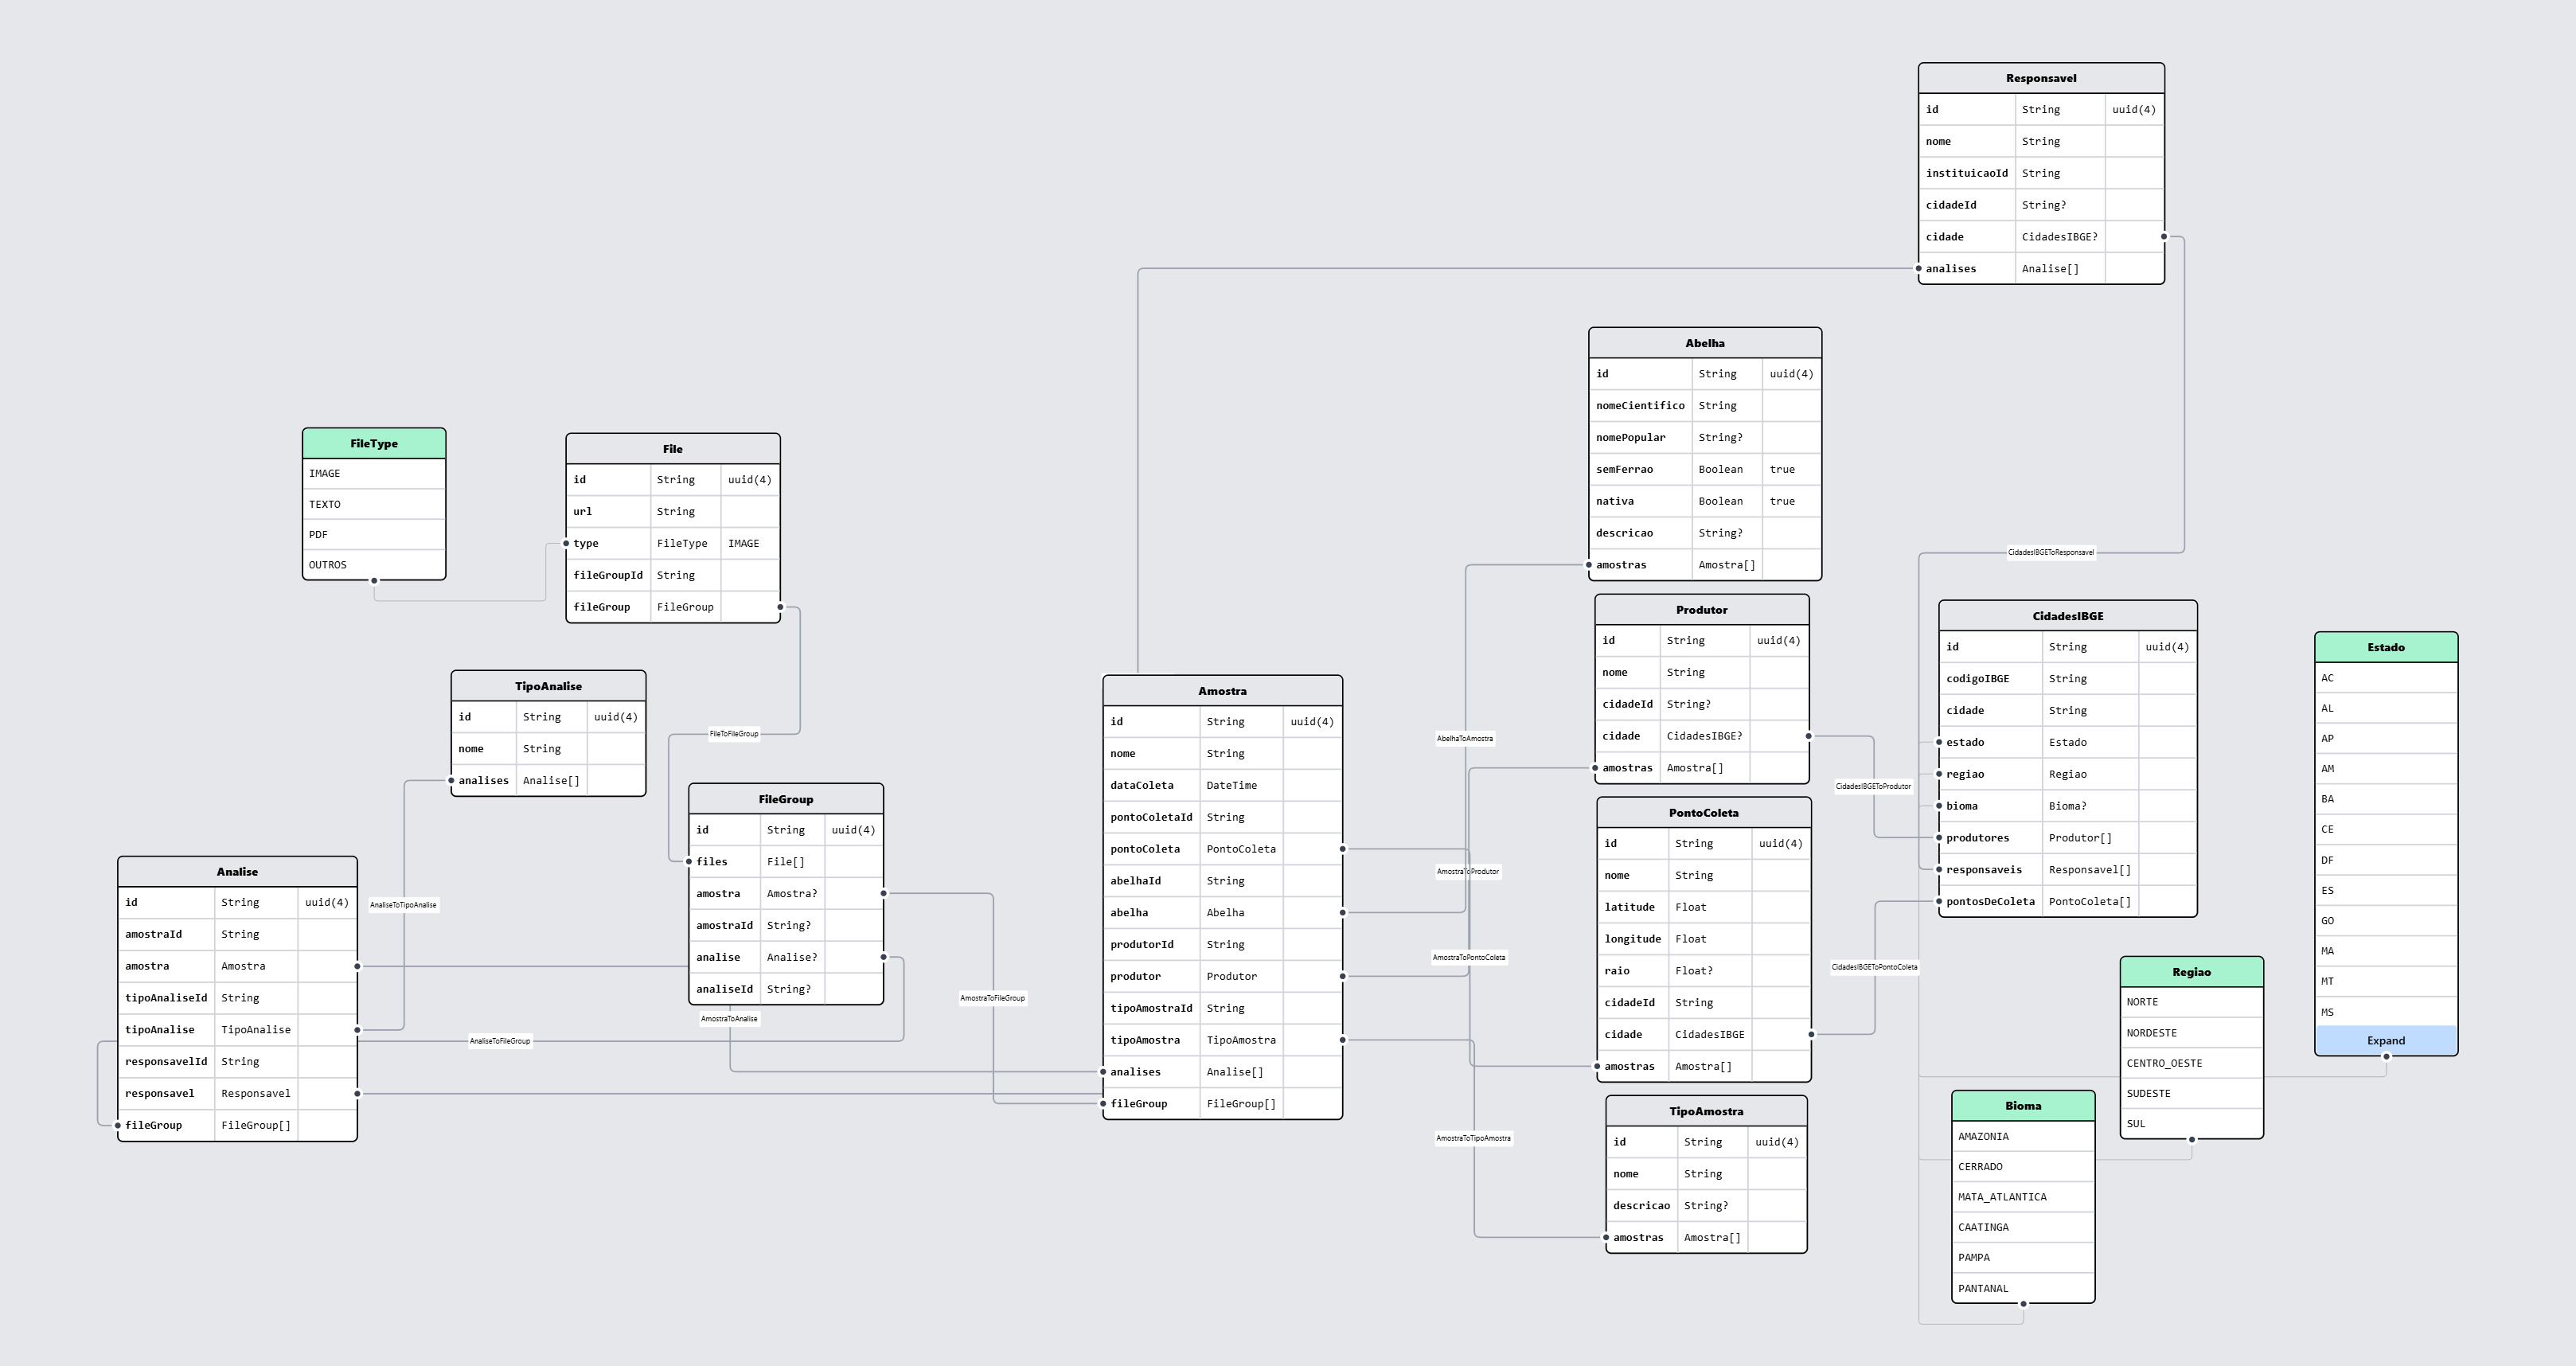
\includegraphics[width=1.0\textwidth]{Imagens/diagramaDB.png}
    \fonte{Autoria própria (2025).}
    \label{fig:der}
\end{figure}

\chapter{Cronograma de Desenvolvimento}

O desenvolvimento da Plataforma de Gerenciamento de Amostras e Análises de Abelhas será executado ao longo do próximo semestre letivo, correspondendo à disciplina de Trabalho de Conclusão de Curso 2 (TCC 2). O planejamento foi estruturado para garantir a entrega incremental de valor, seguindo os princípios ágeis adotados na metodologia.

As atividades foram divididas em fases lógicas, desde a configuração do ambiente até a validação final com usuários e defesa do trabalho.

\begin{table}[ht]
\centering
\caption{Cronograma de Atividades Previsto para o TCC 2}
\label{tab:cronograma}
\vspace{0.2cm}
\resizebox{\textwidth}{!}{% Redimensiona a tabela para caber na largura da página
\begin{tabular}{|l|c|c|c|c|c|c|}
\hline
\textbf{Atividades / Mês} & \textbf{Mês 1} & \textbf{Mês 2} & \textbf{Mês 3} & \textbf{Mês 4} & \textbf{Mês 5} & \textbf{Mês 6} \\ \hline
Revisão e Refinamento de Requisitos & X & & & & & \\ \hline
Configuração do Ambiente (Docker/CI) & X & & & & & \\ \hline
Implementação do Banco de Dados & X & X & & & & \\ \hline
Desenvolvimento do Backend (API) & & X & X & & & \\ \hline
Desenvolvimento do Frontend (React) & & & X & X & & \\ \hline
Integração e Testes Unitários & & & & X & X & \\ \hline
Escrita da Monografia Final & & X & X & X & X & \\ \hline
Revisão Final e Preparação da Defesa & & & & & & X \\ \hline
\end{tabular}%
}
\par
\vspace{0.2cm}
\small{Fonte: Autoria própria (2025).}
\end{table}

\section{Detalhamento das Etapas}

\begin{itemize}
    \item \textbf{Mês 1 (Fundação):} Foco na infraestrutura DevOps. Configuração dos containers Docker para o banco de dados PostgreSQL e o sistema de arquivos MinIO. Criação das migrações iniciais do Prisma ORM.
    \item \textbf{Mês 2 e 3 (Core Backend):} Desenvolvimento dos microsserviços principais em Node.js. Implementação da autenticação, gestão de perfis de usuário e CRUD de amostras.
    \item \textbf{Mês 4 (Frontend e Integração):} Construção das interfaces em React. Integração com a API REST. Implementação da funcionalidade de upload de laudos.
    \item \textbf{Mês 5 (Refinamento):} Testes de ponta a ponta, correção de bugs (polimento) e finalização da escrita acadêmica.
    \item \textbf{Mês 6 (Conclusão):} Entrega da versão final do documento e apresentação para a banca examinadora.
\end{itemize}
